% 10 to 15 pages
% talk about various aspects of system's implementation and
% how it is integrated with the interactive technology
% - talk about the sensors and the fuzzy framework for emotion recognition
% and connect that to the game design elements

\section{Recognizing Emotion} %revision: 0
Heart rate (HR), blood pressure, respiration, electrodermal activity (EDA) and galvanic skin response (GSR), as well as facial EMG (Electromyography) are of physiological variables correlated with various emotions most. Interpreting physiological measures into emotion state can be difficult, due to noisy and inaccurate signals, however recent on-going studies in this area by Mandryk and Atkins ~\cite{mandryk2007fuzzy} presented a method to continuously identifying emotional states of the user while playing a computer game. Using the dimensional emotion model and the fuzzy logic, based on a set of physiological measures, in its first phase, their fuzzy model transforms GSR, HR, facial EMG (for frowning and smiling) into arousal and valence variables. In the second phase another fuzzy logic model is used to transform arousal and valence variables into five basic emotion states including: boredom, challenge, excitement, frustration and fun. Their study successfully revealed self-reported emotion states for fun, boredom and excitement are following the trends generated by their fuzzy transformation. The advantage of continuously and quantitatively assessing user's emotional state during an entire play by their fuzzy logic model is what makes their model perfect to be in incorporated with real-time play technologies. Therefore exposing user's emotional state as a new class of unconscious inputs to the play technology.

\section{Affect Engine} %revision: 2
Affect Engine is the software unit developed to transform collected physiological data to their equivalent emotional state in real-time. While it is generally agreed that emotions comprise three components: subjective experience (e.g. feeling joyous), expressive behavior (e.g. smiling), and physiological activation (e.g. arousal) ~\cite{scherer1993neuroscience}, Affect Engine provides a framework for transformation of physiological activations and some expressive behaviors. Affect Engine consists of four major components (Sensor Module, Fuzzification Module, Administration Panel and Engine Proxies), Figure \ref{fig:affect-engine} is a schematic view of these components working together.

\begin{figure}[h!]
  \caption[Affect Engine]
  {Affect Engine}
  \centering
  
\includegraphics[width=0.5\textwidth]{images/placeholder.png}
  \label{fig:gsr-attached}
\end{figure}

At the following a brief description on these components is provided.

\subsection{Sensor Module} %revision: 3
The sensor module consists of a Thought Technology ProComp Infinity encoder ~\cite{tt2013procomp} Figure ~\ref{fig:encoder}, connected to PC with a USB cable, SensorLib as the basic application programming interface (API) receives raw physiological inputs from the encoder driver and provides functionalities to apply different filters such as low-pass, high-pass, smoothing and shifting to the signal.

\begin{figure}[h!]
  \caption[Thought Technology ProComp Infinity Encoder]
  {Thought Technology ProComp Infinity encoder}
  \centering
  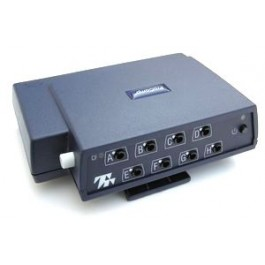
\includegraphics[width=0.5\textwidth]{images/encoder.png}
  \label{fig:encoder}
\end{figure}

\subsection{Fuzzification Module} \label{subsec:fuzzi} %revision: 3
Then filtered signals are fuzzified by the use of a set of fuzzy rules in the first phase of transformation. Then generated arousal and valence values are transformed into emotion values using another set of fuzzy rules in the second pass ~\cite{mandryk2007fuzzy}. A sample set for fuzzy rules used in the first and the second phase can be found in Appendix ~\ref{app:phys-to-av} and ~\ref{app:av-to-emotion}. Appliactions such as games can easily integrate the system where emotion recognition can offer adaptive control to maintain user interest and engagement. Once connected via sensors to the emotion recognition system, the affective state of the user can be captured continuously and in real-time and it can be monitored on a displayed 2-dimenstional graph of valance and arousal, Figure 1.


\subsection{Administration Panel}

\begin{figure}[h!]
  \caption[Administration Panel]
  {Administration Panel}
  \centering
  
\includegraphics[width=0.5\textwidth]{images/placeholder.png}
  \label{fig:administration-panel}
\end{figure}

\subsection{Engine Proxies}

\section{Sensors}

Currently the system uses Blood Volume Pulse (BVP), Galvanic Skin Response (GSR) and Electromyography (EMG; for frowning and smiling), to classify human affective states in 2-dimensional valence/arousal space, Figure 2. The system has three modules, Figure 4:

The Blood Volume Pulse (BVP) signal is a relative measure of the amount of blood owing in a vessel. From BVP we calculated heart rate and heart rate variability. The heart rate is known to re ect emotional activity and has been used to differentiate between both negative and positive emotions as well as different arousal levels ~\cite{tt2013procomp} The Galvanic Skin Response (GSR) sensor to measure the skin's conductance (between two electrodes and is a function of sweat gland activity and the skin's pore size). As a person becomes more or less stressed, the skin's conductance increases or decreases proportionally ~\cite{picard2003affective}.

\subsection{Heart Rate}
\subsection{Galvanic Skin Response}
\subsection{Facial Electromyography}


\section{Inegration with Valve Source Engine}
% talk about Modding Half Life EP2
\subsection{Level Design}
\subsection{The Director}
